\chapter{Introducción y wavelets ortogonales }
\columnratio{0.7,0.3}
\setlength{\columnsep}{1cm} % Ajusta el espacio entre las columnas a 1cm

\begin{paracol}{2}
Sea $f=\left(f_1,\ldots,f_N\right)\in \mathbb{R}^N$$, N=2^k$, con $k$ Máximo nivel de descomposición. La energía viene dado por:
$$E(f)=\sum_{j=0}^{N}f_j^2=\|f\|^2.$$
Una aproximación $A$ a primer nivel viene dado por el promedio de la primera y segunda pareja de términos. Es decir, se aproxima a la señal original. Y el detalle $D$ viene dado por la diferencia de la primera y segunda pareja de términos. Es decir, aquello que necesito añadir para recuperar la señal original. 

Cuando se tiene una aproximación de último nivel la señal se queda plana, por ejemplo:
$$A^2(3.75,3.75,3.75,3.75).$$
En este caso, como las entradas son, $k=2$, en consecuencia $2^2=4$, solo se puede realizar dos niveles de aproximación. 

Ahora bien para entender de mejor manera el concepto de wavelets necesitamos recordar las siguientes definiciones de algebra lineal:
\switchcolumn[1]*{\noindent\scriptsize
	\begin{itemize}
	    \item Si tenemos un sistema ortonormal, cualquier elemento que sea combinación lineal es fácil obtener los coeficientes. Es decir, no hay que resolver un sistema de ecuaciones.
	    \item La proyección ortogonal es el punto más cercano a un subespacio. 
	    \item Si yo hago la imagen de dos vectores el producto de las imágenes es igual al producto de las entradas. 
	    \item La norma de partida sea igual a la norma de llegada. Es decir, es transformación ortonormal si conserva la energía.
	\end{itemize}
}
\switchcolumn[0]
\begin{itemize}
    \item Si $\left\{v_1,\ldots,v_m\right\}\subset \mathbb{R}^N$, la envoltura lineal de dicho conjunto de vectores en $lin\left\{v_1,\ldots,v_m\right\}$.
    \item Si $v,w\in\mathbb{R}^N$, su producto escalar es $v\cdot w = v_1w_1+\ldots+v_Nw_N$.
    \item Un sistema de vectores $\left\{v_1,\ldots,v_m\right\}$ es ortonormal si cada uno tiene norma $1$ y $v_i\cdot v_j=0$ para $i\neq j$. En ese caso, cada vector $u\in lin\left\{v_1,\ldots,v_m\right\}$ se expresa de forma única como $u=(u\cdot v_1)v_1+\cdots + (u\cdot v_m)v_m$.
    \item Dos subespacios $V,W\subset \mathbb{R}^N$ son ortogonales si cada elemento de $V$ es ortogonal a cada uno de $W$, y su suma es directa (y ortogonal), la cual denotamos por $V\oplus^\perp W$.
    \item Si $v\in \mathbb{R}^N$ y $W$ es un subespacio de $\mathbb{R}^N$, la proyección ortogonal $w$ de $v$ sobre $W$ es el único vector $w\in W$ tal que $v-w$ es ortogonal a $W$ (y coincide con el de mínima distancia en $W$ a $v$).
    \item Una aplicación lineal $T:\mathbb{R}^N \to \mathbb{R}^N$ es una transformación ortogonal si $Tu\cdot Tv=u\cdot v$ para $u,v\in \mathbb{R}^N$ arbitrarios (equivalencia a $\|Tu\|=\|u\|$ para todo $u$). También, que su expresión matricial en una base ortonormal sea una matriz $A$ ortogonal ($A\cdot A^T=I$).
\end{itemize}

\section{Wavelets de Haar}
Cuando se toma el sistema
$$\left\{v_1^1,\ldots,v_{N/2}^1,w_1^1,\ldots,w_{N/2}^1\right\}$$
de scaling y Wavelets, si se proyecta en el espacio de la scaling la proyección me sale $A^1$, y si proyecto ortogonalmente en el espacio de Wavelets la proyección me sale $D^1$. En otras palabras,
$$
\begin{array}{rcl}
    f&=&\left((f_1\cdot v_1^1)v_1^1+\cdots+(f_{N/2}\cdot v_{N/2}^1)v_{N/2}^1\right)\\\\
     &+& \left((f\cdot w_1^1)w_1^1+\cdots+(f\cdot w_{N/2}^1)w_{N/2}^1\right)\\\\
     &=&A^1+D^1.
\end{array}
$$
De esta manera, el espacio scaling a nivel 1 es la envoltura lineal de $v_1^1,\ldots,v_{N/2}^1$ y el espacio Wavelets a nivel 1 es la envoltura lineal de $w_1^1,\ldots,w_{N/2}^1$. Dado que scaling y wevelets son perpendiculares entre si, la suma directa de estos dos espacios nos da:
$$\mathbb{R}^N = V^1\oplus^\perp W^1.$$
Con $V$, $\dim N/2$ y $W$ $\dim N/2$.

Cuando vamos al siguiente nivel, la parte de detalles no las toco, si no que me fijo en la parte de aproximación. Y ese espacio lo vuelvo a partir en dos.De lo que sale:
$$V^1 = V^2\oplus^\perp W^2.$$
con $V^2$, $\dim N/4$ y $W^2$ $\dim N/4$.
Por lo tanto,
$$\mathbb{R}^N = V^2\oplus^\perp W^2\oplus^\perp D^1.$$

Los coeficientes son los productos escalares. 

Coleccionar las subseñales es de lo que consiste la tranformada de Haar. 

Las señales de aproximación $A$ se le llama también señales de tendencia y a las señales $D$ de detalle se le llama fluctuaciones.


\section{Wavelets de Daubechies (db2)}
En vez de utilizar 2 coeficientes, se utilizan 4 coeficientes en la parte de scaling y 4 coeficientes en la parte de Wavelets.

Ganamos en comparación de Haar, la compactación de energía.


\end{paracol}


\chapter{Análisis de Frecuencia}

\begin{paracol}{2}
Las Transformadas Wavelet tiene un reflejo en la frecuencia por lo que recordaremos como es la Transformada de Fourier.

\section{Análisis de la frecuencia en la Transformada Wavelet (DFT)}

Notación:
$$f=\left(f(0),f(1),\ldots,f(N-1)\right)\in \mathbb{R}^N.$$

\switchcolumn[1]*{\noindent\scriptsize
Geométricamente,
\begin{center}
    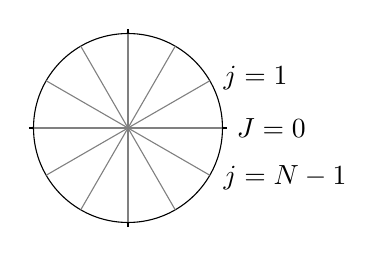
\begin{tikzpicture}[scale=.6]
	% Dibujar los ejes
	\draw[thick] (-2.1,0) -- (2.1,0);
	\draw[thick] (0,-2.1) -- (0,2.1);

	% Dibujar el círculo
	\draw (0,0) circle (2cm);

	% Dibujar los ángulos
	\foreach \x in {0,30,...,360} {
	    \draw[gray] (0,0) -- (\x:2cm);
	}

	% Etiquetar los ángulos
	\foreach \x/\xtext in {
	    0/J=0,
	    30/j=1,
	    330/j=N-1
	} {
	    \draw (\x:2.1cm) node[right]{$\xtext$};
	}
    \end{tikzpicture}
    \begin{itemize}
	\item Tomamos como entrada vectores en $\mathbb{R}$ y nos devuelve vectores en $\mathbb{C}$.
    \end{itemize}
\end{center}
}
\switchcolumn[0]
De lo que la transformada discreta de Fourier lo definimos como:
\begin{equation}
\hat{f}(k)=\sum_{j=0}^{N-1}f(j)e^{-i2\pi kj/N}, \quad k=0,1,\ldots,N-1.
\end{equation}

Comenzamos en $0$ debido a que $e^0=1$. Luego voy corriendo una posición cada vez el circulo en $N$ trozos. Cuando tenemos $j=1$. Entonces, $e^{-i2\pi k/N}$.

Ahora, la inversa de la transformada de Fourier está definida como:
\begin{equation}
    f(j)=\frac{1}{N}\sum_{k=0}^{N-1}\hat{f}(k)e^{i2\pi kj/N}, \quad j=0,1,\ldots,N-1.
\end{equation}

Otra de las propiedades de la transformada de Fourier es periódica. Es decir, para $k=N$, el ciclo se repite. Dado que, 
$$e^{i2\pi kj/N}=e^{i2\pi Nj/N}=e^{i2\pi j}=e^0=1.$$
Por la igualdad de Parseval, sabemos que la energía mas o menos se conserva. Es decir,
\switchcolumn[1]*{\noindent\scriptsize
    \begin{itemize}
	\item Cuando tomamos la energía $E(\hat{f})$ que serán números complejos, no tomamos los cuadrados de las entradas, si no los cuadrados de los módulos de las entradas.
    \end{itemize}
}
\switchcolumn[0]\noindent
$$E(f)=\dfrac{1}{N}E(\hat{f}).$$

\subsection{Implementación computacional}
Vemos que (1.1) tiene $N$ multiplicaciones para $N$ entradas $k$. Donde si aplicamos computacionalmente, se tiene un costo de orden de $N^2$. Por lo que, se tiene un costo computacional alto. Por lo tanto, usamos la trasformada rápida de Fourier (FFT). La cual tiene un costo computacional de $N\log N$.

Luego, para visualizar las señales de la transformada de Fourier, usamos el espectro de la señal. Es decir, consideramos los módulos al cuadrado de las entradas $|\hat{f}|^2$. La energía de $f$ resulta ser el valor medio del espectro
$$E(f)=\dfrac{1}{N}\sum_{k=0}^{N-1}|\hat{f}(k)|^2.$$

Que es la media del espectro, dado por:
$$\left(|\hat{f}(0)|^2+|\hat{f}(1)|^2+\ldots+|\hat{f}(N-1)|^2\right).$$

\switchcolumn[1]*{\noindent\scriptsize
	\begin{itemize}
	    \item Al descomponer una señal, lo que estoy realizando son proyecciones ortogonales.
	    \item Sabemos que con aproximación numérica se va promediando la energía.
	    \item En tema de detalle es como fluctúan los coeficientes entre si.
	\end{itemize}
}
A partir del espectro podemos analizar el efecto que produce el tratamiento de señales mediante wavelets a nivel de frecuencia.
\switchcolumn[0]
Ahora bien cuando separamos las señales, mediante promedios y diferencias, y aplicamos la transformada wavelet a estas separaciones de $A^1$ y $D^1$. Entonces, en $A^1$ se queda las frecuencias bajas y en $D^1$ las frecuencias altas. Esto se conoce como filtros pasa bajos y pasa altos. Esto lo podemos verificar en general a partir de las formulas de las señales de promedio y detalle y por la linealidad de la transformada de Fourier discreta:
$$A^1 = (f\cdot v_1^1)v_1^1 + \cdots + (f\cdot v^1_{N/2}v^1_{N/2}.$$
$$D^1 = (f\cdot w_1^1)w_1^1 + \cdots + (f\cdot w^1_{N/2}w^1_{N/2}.$$
Aplicando la transformada de Fourier a $A^1$ y $D^1$ se tiene:
$$\hat{A}^1 = (f\cdot v_1^1)\hat{v}_1^1 + \cdots + (f\cdot v^1_{N/2})\hat{v}^1_{N/2} \quad (\text{Deja pasar frec bajas}).$$
$$\hat{D}^1 = (f\cdot w_1^1)\hat{w}_1^1 + \cdots + (f\cdot w^1_{N/2})\hat{w}^1_{N/2} \quad (\text{Dejan pasar las altas}).$$


Ahora para el nivel 2, hago una aproximación promediando más términos por lo que la meseta lo estrecho, es decir mi filtro es de frecuencias más bajas. Recordando la composición de la señal:
$$f = A^2 + D^2 + D^1.$$
Donde $D^1$ ya se tiene la frecuencias altas, $A^2$ tiene las frecuencias bajas y $D^2$ tiene las frecuencias medias o filtro pasa bandas, con
$$A^2=\sum_{j=0}^{N/2-1}f(2j)\hat{v}^2_j,$$ 
pasa bajas y
$$D^2=\sum_{j=0}^{N/2-1}f(2j+1)\hat{w}^2_j.$$
pasa bandas.

\end{paracol}
